\section{Introduction}
In Astronomy, instruments with higher angular resolution allows us to measure ever smaller structures in the sky. For Radio frequencies, the angular resolution is bound to the antenna dish diameter, which puts practical and financial limitations on the highest possible angular resolution. Radio Interferometers get around this limitation by using several smaller antennas instead. Together, they act as a single large antenna with higher angular resolution at lower financial costs compared to single dish instruments.

However, Radio Interferometers do not measure the pixels of the sky image. Instead, Radio Interferometers measure an incomplete set of Fourier components. The sky image has to be reconstructed from the measurements. This forms an ill-posed inverse problem: There are potentially many different images that fit the measurements, and 
from the measurements alone we cannot decide which image was actually observed.

Algorithms that solve the ill-posed Image Reconstruction problem. Find most likely images. Extensive Research in the last decades.

SKA wants to create Radio Interferometers on a new scale.
MeerKAT is the precursor of SKA-Mid. Create a new scale of Fourier measurements.
Push towards distributing
The Image Reconstruction Problem has to be solved with distributed computing.

Algorithms were developed before the advent of distributed computing. 
Distribution so far has been difficult. Only small number of nodes.


Target to distribute the image reconstruction
First tests


\subsection{Radio Interferometry System}\label{intro:sys}
This project is focused on distributing Image Reconstruction for Radio Interferometers, which is only one of three steps in the pipeline from measurements to the final image. We give a quick overview over the whole pipeline in figure \ref{intro:system} and how Radio Interferometers work in principle: The antennas observe the arriving electromagnetic wave, gets processed in three steps, Correlation, Calibration and Image Reconstruction. 

\begin{figure}[h]
	\centering
	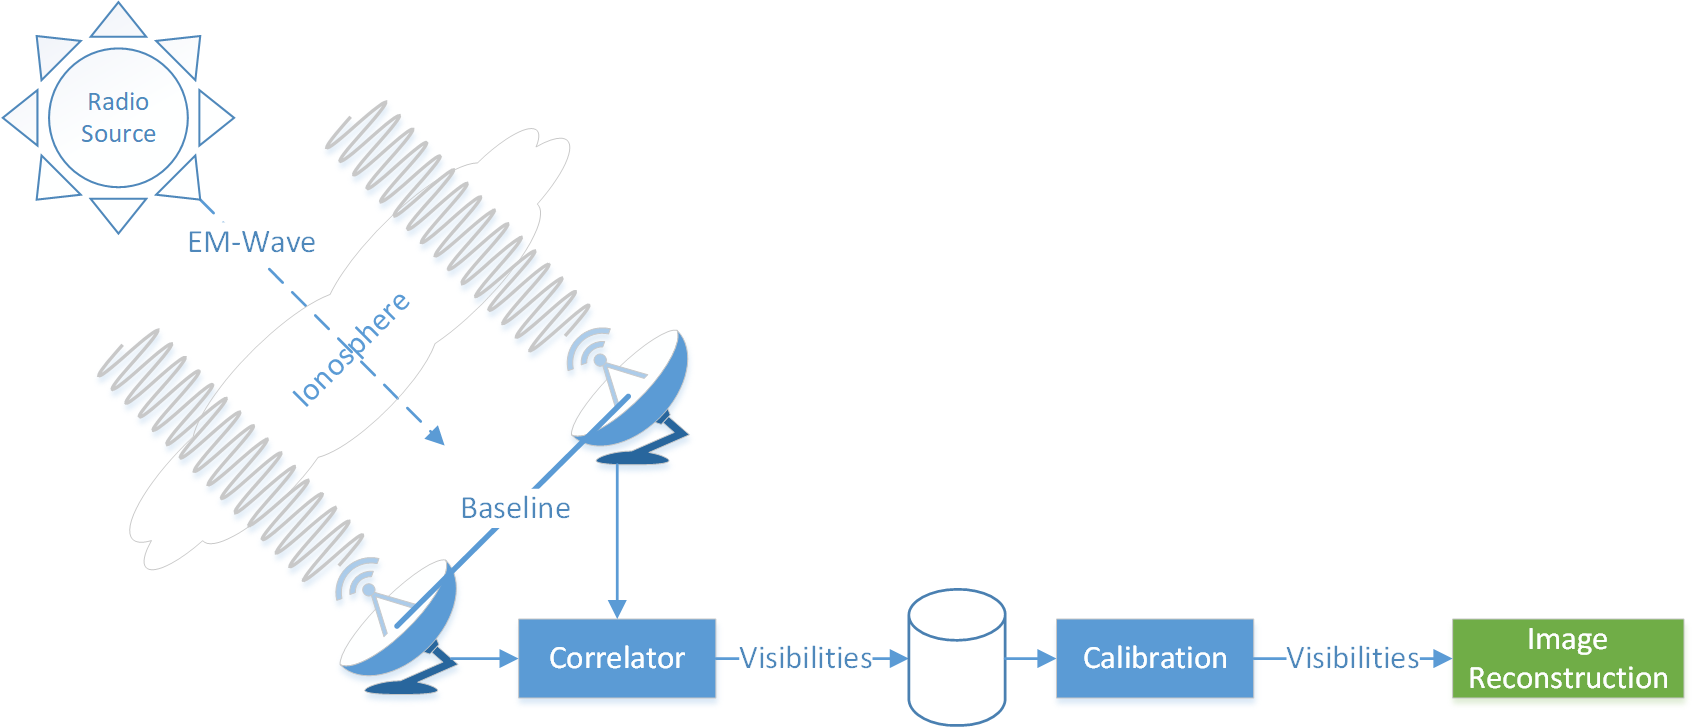
\includegraphics[width=0.80\linewidth]{./chapters/01.intro/system.png}
	\caption{Radio Interferometer System}
	\label{intro:system}
\end{figure}

First, the electromagnetic wave gets measured by the different antennas of the interferometer. The measurements of each antenna pair get correlated into a complex-valued Fourier Component (called Visibility in Radio Astronomy). Each antenna pair measures a noisy amplitude and phase of a single Visibility (Fourier Component) of the sky image. The distance and orientation of the antenna pair relative to the incoming signal, called the baseline, dictates which Visibility gets measured. The longer the baseline the higher-order Visibility gets measured, resulting in a higher angular resolution. After correlation, the Visibility data is saved for later processing.

The Calibration step is done after all Visibility data has been recorded. This step corrects the amplitude and phase of the measurements for varying antenna sensitivities, pointing errors and other effects. Also, this step removes corrupted data from the measurements. After the Visibilities are calibrated, we can average the measurements and reduce the data volume by several factors. Typically, averaging is done to reduce the runtime costs of the Image Reconstruction step.

The Image Reconstruction step takes the calibrated, and potentially averaged down Visibility data and finds the most likely observed image of the sky. Although the Interferometer produces a potentially large number of Visibilities, they are incomplete: For example an Interferometer with dish-antennas is typically blind to the microwave background radiation. The largest structures in the image it can detect depends on the shortest baseline. Since the antennas have to be at least the dish-diameter placed apart, the Interferometer is simply blind to very large structures in the sky image, like the microwave background radiation. This property makes Image Reconstruction Problem ill-posed. In the Image Reconstruction step, we therefore have to find the most likely image which fits the measurements.

\subsubsection{Earth's rotation and arbitrary large Number of Visibilities}
To improve the final image, we want to measure as many different Visibilities as possible. Modern Radio Interferometers use the the earth's rotation to change the baselines. When the earth rotates, it modifies the length of the baseline and by extent, what Visibilities get measured. Modern Interferometer can produce an almost arbitrary large number of measurements by just increasing the observation time.

The data volume can be averaged down in the Calibration step. However, with self-calibration, the Image Reconstruction is tasked with solving both the most likely image and the calibration parameters at the same time. This further improves the reconstruction quality\cite{Wiauxselfcal}, but requires the Image Reconstruction step to handle all the Visibility data.

Modern Radio Interferometers can produce an almost arbitrary large number of measurements. The reconstruction quality benefits from a large number of different Visibility measurements. The two main limiting factors however, are the cost of data storage and the scalability of the Image Reconstruction algorithm.


\subsection{The Image Reconstruction Problem}
For Radio Interferometers, Image Reconstruction forms an ill-posed inverse problem. There are potentially many different images that fit the measurements. The Image Reconstruction is tasked with finding the most likely image $I()$ given the (calibrated) Visibility measurements $V()$.  Figure \ref{intro:inversefig} shows an example from a MeerKAT observation for $V()$ and $I()$. The image \ref{intro:inversefig:uvspace} shows the incomplete sampling in the Fourier space. The sample density decreases away from the center\footnote{The center has actually no samples, since the MeerKAT Radio Interferometer uses antenna's with dishes. Due to the resolution, it might not be visible in the image \ref{intro:inversefig:uvspace}.}. The observed image \ref{intro:inversefig:reconstruction} contains two classes of structure, point sources and extended emissions. Point sources arise from stars and other distant objects, their emissions are concentrated around a single pixel. Extended emissions arise from hydrogen clouds and other sources which span an area of several arc-seconds of the sky.

\begin{figure}[htp]
	% preliminary
	\sbox\twosubbox{%
		\resizebox{\dimexpr.9\textwidth-1em}{!}{%
			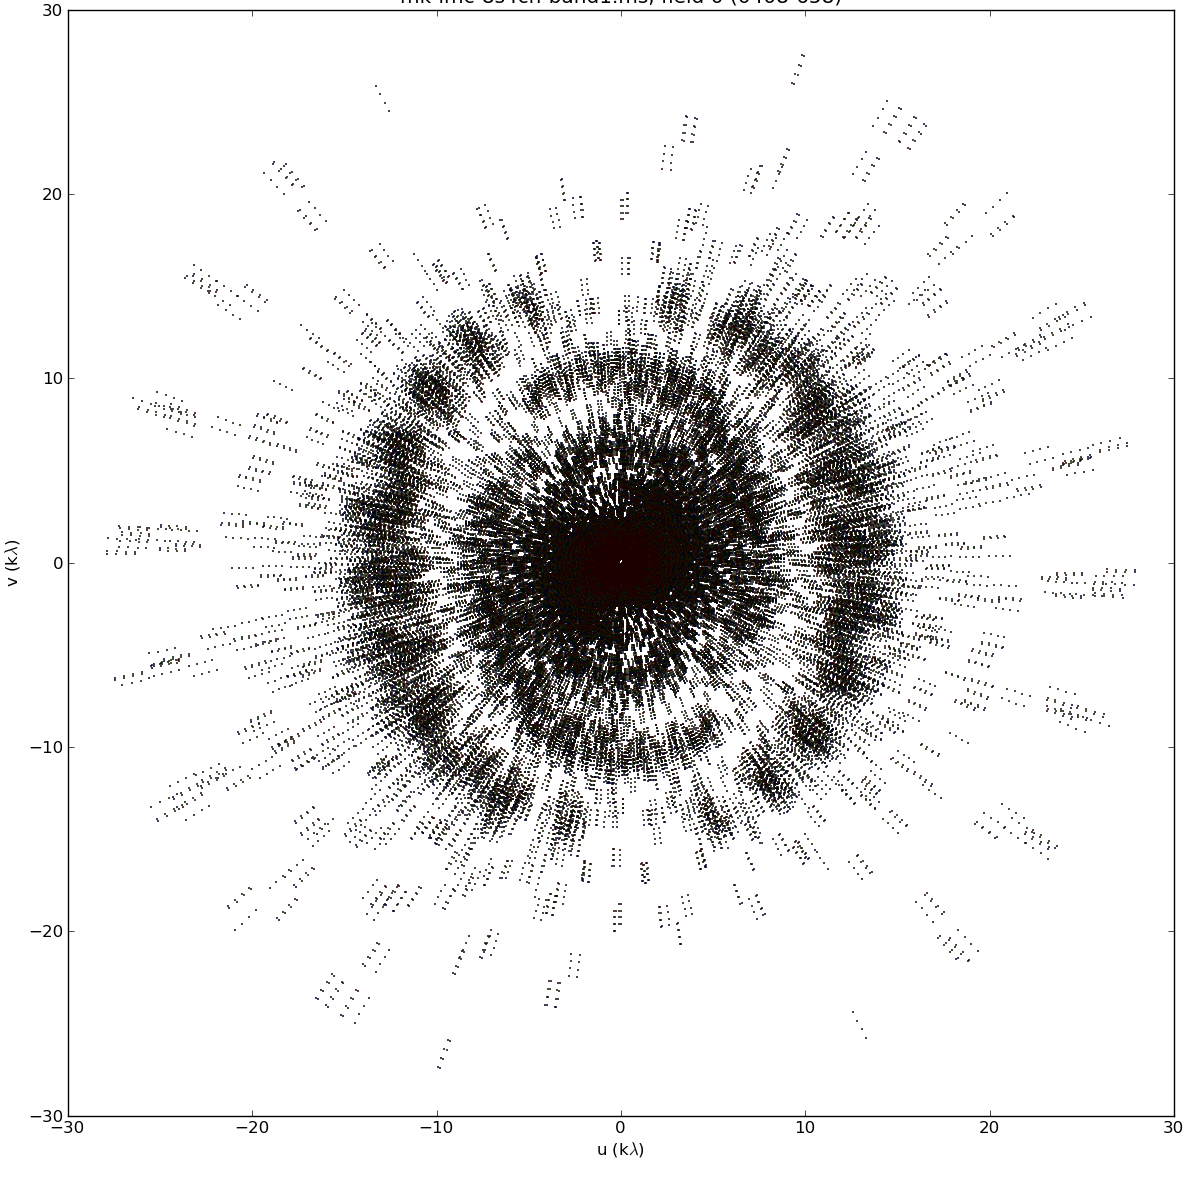
\includegraphics[height=3cm]{./chapters/01.intro/meerkat_uv2.png}%
			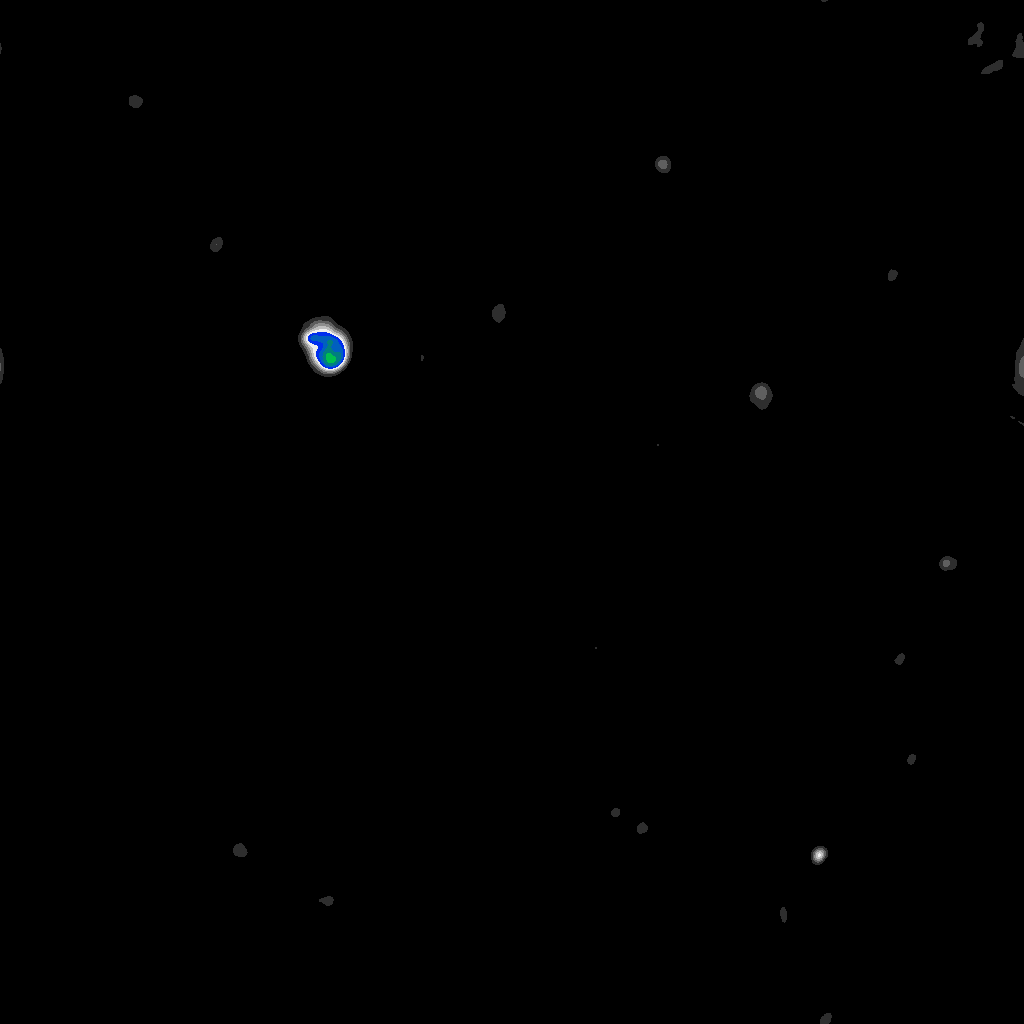
\includegraphics[height=3cm]{./chapters/01.intro/mk2/clean.png}%
		}%
	}
	\setlength{\twosubht}{\ht\twosubbox}
	
	% typeset
	\centering
	\subcaptionbox{Measurements $V()$ in the $uv$-plane.\label{intro:inversefig:uvspace}}{%
		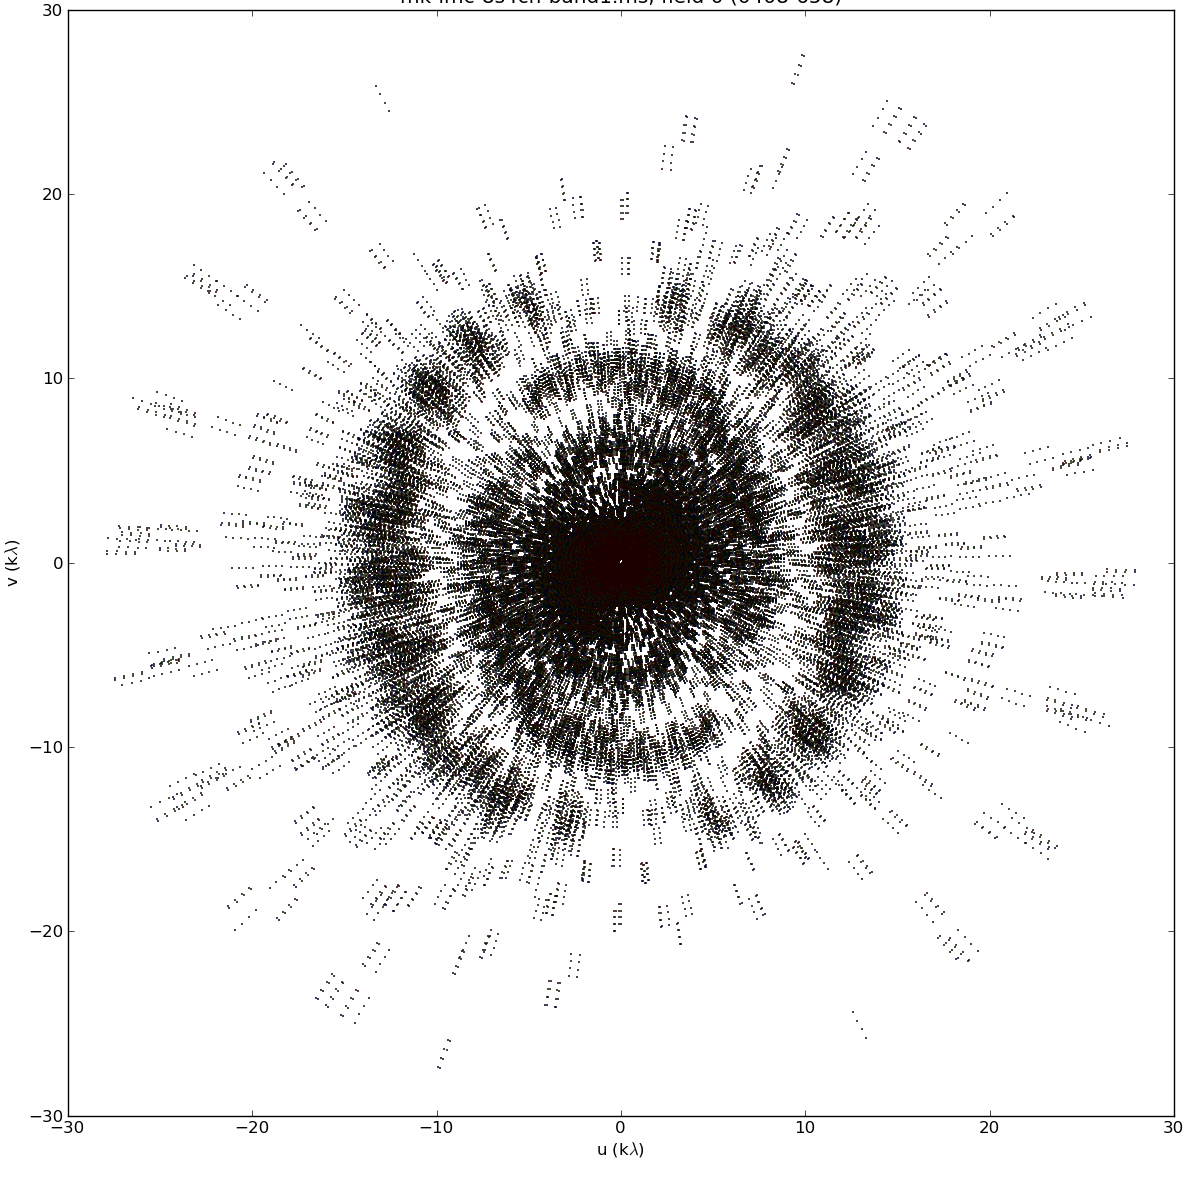
\includegraphics[height=\twosubht]{./chapters/01.intro/meerkat_uv2.png}%
	}\quad
	\subcaptionbox{The observed image $I()$.\label{intro:inversefig:reconstruction}}{%
		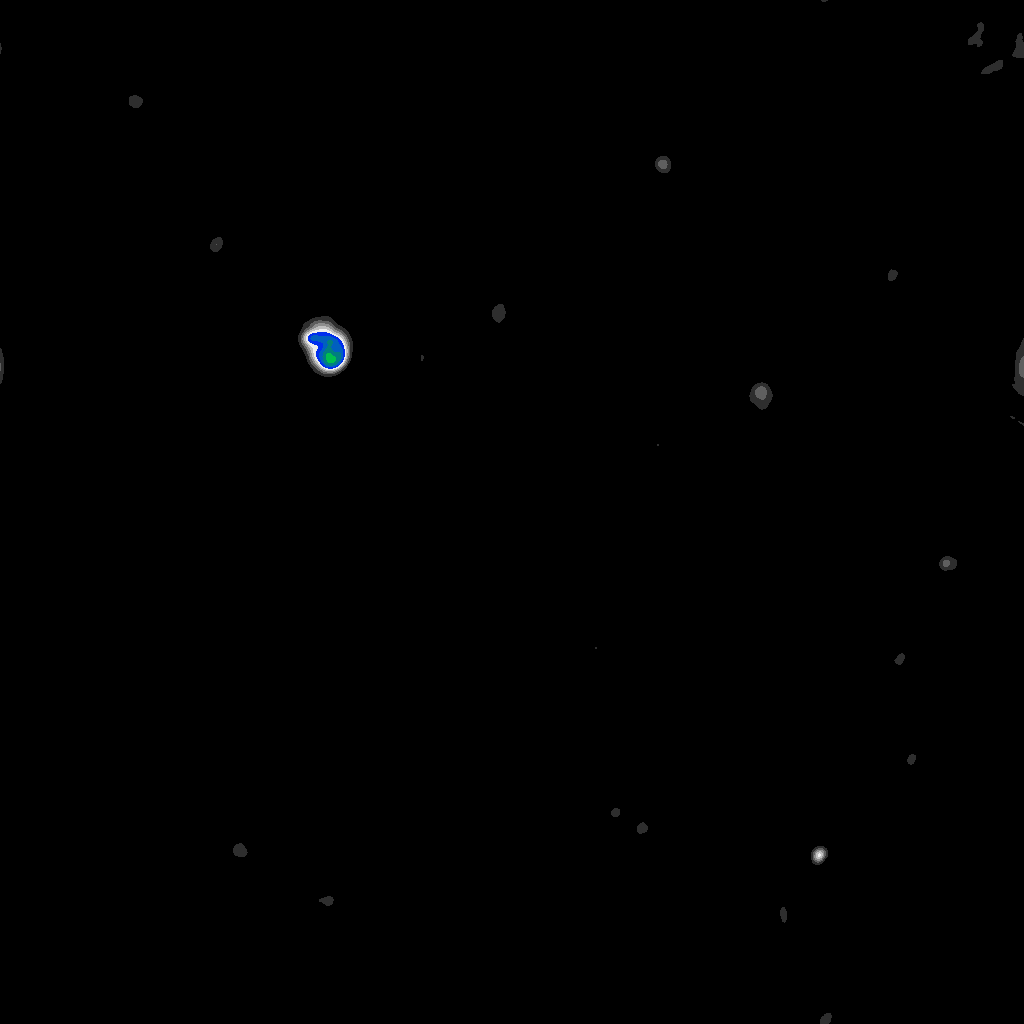
\includegraphics[height=\twosubht]{./chapters/01.intro/mk2/clean.png}%
	}
	\caption{The Image Reconstruction Problem}\label{intro:inversefig}
\end{figure}

Formally, we want to invert the measurement equation of the Radio Interferometer.

Equation \eqref{intro:inverseproblem} shows a measurement equation for Radio Interferometers, 


\begin{equation}\label{intro:inverseproblem}
V(u, v, w) = \int\int  \frac{I(x, y)}{c(x, y)}  e^{2 \pi i [ux+vy+ w(c(x, y) - 1)]} \: dx \: dy \:,  \quad c(x,y) = \sqrt{1 - x^2 - y ^2}
\end{equation}

The measurement equation \eqref{intro:inverseproblem} contains three parts. The Visibility measurements $V(u,v,w)$, the observed image with a normalization factor $\frac{I(x, y)}{c(x, y)}$ and the Fourier Transform $e^{2 \pi i [\ldots]}$. The $x$ and $y$ coordinates are angles from the image center. A pixel in $I(x,y)$ represents how much radio emission was measured from a the direction $x,y$. Note that the Visibilities $V(u,v,w)$ are three dimensional, while the image $I(x,y)$ only has two. However, also note that the third component $w$ only depends on the directions $x$ and $y$. In a sense, the Visibilities $V()$ and the Image $I()$ have a two dimensional Fourier relationship ($V(u,v,w) = \int\int I(x,y) e^{2 \pi i [ux+vy]} \: dx \: dy$), but with a directionally dependent correction factor $e^{2 \pi i [\ldots +w(c(x, y) - 1)]}$. 

The third component $w$ is an example of a Directionally Dependent Effect (DDE) which have a tendency to increase the runtime costs of the Image Reconstruction. The $w$-component keeps us from using the Fast Fourier Transform (FFT) for the measurement equation \eqref{intro:inverseproblem}. Research in this area tries to use approximations which lets us use faster algorithms like the FFT, and correct for DDE's accurately enough \cite{veenboer2017image, offringa2014wsclean, pratley2018fast}. In this project, the $w$-correction is the only DDE we handle.

\subsubsection{System of Linear Equations}\label{intro:linear}
Even though the Fourier Transform in equation \eqref{intro:inverseproblem} contains a $w$-correction factor, $V()$ and $I()$ have still a linear relationship. This means we can represent the Image Reconstruction Problem as a system of linear equations: \eqref{intro:linear:linear}. $F$ is the Fourier Transform with $w$-correction, $x$ is the image we are searching and $V$ are the measured Visibilities\footnote{$V$ in the equation \eqref{intro:linear:linear} is a vector. We use the lower-case $v$ to denote the axis in the Fourier space $uvw$, and the upper-case letter to denote the Visibility vector.}.

\begin{equation}\label{intro:linear:linear}
\underset{x}{find}\quad V = Fx
\end{equation}

As we discussed in section \ref{intro:sys}, Radio Interferometers can produce an almost arbitrary large number of Visibilities. In practice, we often reconstruct images with far fewer pixels than Visibility measurements, making the equation \eqref{intro:linear:linear} an over-determined problem. Meaning equation \eqref{intro:linear:linear} is either consistent and has a unique solution $x$, or is inconsistent with no solutions. Sadly, the Visibility measurements are subject to noise. The equation \eqref{intro:linear:linear} is inconsistent does not have a solution. To solve the Image Reconstruction Problem, we need to account for noise in the measurements, which leads us to a new inequality \eqref{intro:linear:l2}.

\begin{equation}\label{intro:linear:l2}
\underset{x}{find} \: \left \| V - Fx \right \|_2^2 < \epsilon
\end{equation}

We use the L2 norm and find the solution $x$ which, when the Fourier Transform is applied, has the smallest distance to the measurements $V$. The L2 norm leads to a strictly-convex function, meaning \eqref{intro:linear:l2} has only one minimum, and we can use convex optimization techniques to find it. So the question arises, is the observed image $I()$ located at the global minimum of \eqref{intro:linear:l2}? Although we have more measurements than pixels in the reconstruction, the set of Visibilities are still incomplete. They shift the observed image some distance away from the global minimum of \eqref{intro:linear:l2}. From the measurements alone, we cannot locate the observed image. We know it is near the global minimum, but we do not know where it is. The equation \eqref{intro:linear:l2} has many candidate solutions $x$, one of which is the observed image.  From the measurements alone, we cannot decide which candidate was the observed image, and \eqref{intro:linear:l2} is an ill-posed inverse problem. 

Intuitively, the incomplete measurements allow the pixels $x$ in the reconstruction to form physically implausible solutions. 

In many Image Reconstruction Problems of Radio Interferometry, the pixels cannot be negative.
We know it contains stars, 

 If we include prior information about the image, we can retrieve the most likely image from all the candidates of \eqref{intro:linear:l2}.
The question is, what are the chances that the most likely image is the observed image?
The theory of Compressed Sensing tells us this.

\subsubsection{Theory of Compressed Sensing}
Theory of Compressed Sensing \cite{candes2006robust, donoho2006compressed} is a recently developed sampling theorem.
How we can include prior information about the image and how likely we are to retrieve the observed image. 
Prior.

sparsity
Dictionary $D$. For example Wavelets. Can be larger than the number of pixels

For our considerations LASSO objective \eqref{intro:linear:compressed:lasso}

\begin{equation}\label{intro:linear:compressed:lasso}
\underset{x}{minimize} \: \left \| V - Fx \right \|_2^2 + \lambda \left \| D^{-1}x \right \|_1 
\end{equation}

Data term
Regularization term

Problem of a result: we still don't know how close we are, or if certain structures

So we need a Regularization Dicitionary $D$, which captures the prior information we have about the image. Then, we can use convex optimization techniques to minimize the objective \eqref{intro:linear:compressed:lasso}.






\subsubsection{Different Representations for the LASSO Objective}

There are different ways to represent the LASSO objective \eqref{intro:linear:compressed:lasso}. Has the data term in the Fourier space, and reconstructs the image directly. We have different design decisions here. We can choose the Data term to be either in Fourier or image space, and we can set the Variables to be in either image, uniform Fourier or in the sparse space.

These possibilities arise from the Fourier Transform Matrix $F$, shown in equation \eqref{intro:linear:repr:fourier}. The first line shows the normal Fourier transform, from image $x$ into Visibilities $V$. Since $x$ is in a uniformly-sampled space, we can factorize $F$ into the FFT and the masking matrix $M$ and we arrive at the second line of equation \eqref{intro:linear:repr:fourier}. $M$ is essentially a matrix contains values between zero and one.
Represents the degradation due to incomplete measurements. 

\begin{equation} \label{intro:linear:repr:fourier}
\begin{split}
V &= Fx\\
V &= M\: FFT(x)\\
V &= M\: V_2\\
I_{Dirty} &= x \star PSF
\end{split}
\end{equation}

We can use the matrix $M$ directly, and use it to transform from uniformly sampled Visibilities $V_2$ to non-uniformly sampled Visibilities $V$, arriving at line three of equation \eqref{intro:linear:repr:fourier}.

Since a multiplication in Fourier space is a convolution in image space, we can also represent the masking matrix $M$ as a Point Spread Function $PSF$ in image space. Degradation is a convolution.

All these lines are of \eqref{intro:linear:repr:fourier} all represent the Image Reconstruction Problem in different spaces. For example, if we change the data term in our LASSO objective from $\left \| V - Fx \right \|_2^2$ to a deconvolution $\left \| I_{Dirty} - x \star PSF \right \|_2^2$ we arrive at the same global minimum. But, in Radio Astronomy, the images are magnitudes smaller than the calibrated Visibility measurements $V$. 
Potential to reduce the costs. 
In practice, we have an accuracy issue with the $PSF$, since it is not constant. The $PSF$ changes over the image due to DDEs like $w$-correction.

We can set the data term in our LASSO objective to either Visibility or image space. The reconstruction space has three possible design choices, which leads to three different LASSO objectives.

\begin{alignat}{2}
\text{analysis:}\: \underset{x}{minimize}\:& \left \| V - Fx \right \|_2^2 + &\lambda \left \| D^{-1}x \right \|_1  \\
\text{in-painting:}\: \underset{V_2}{minimize}\:& \left \| V - MV_2 \right \|_2^2 + &\lambda \left \| D^{-1}F^{-1}V_2 \right \|_1  \\
\text{synthesis:}\: \underset{\alpha}{minimize}\:& \left \| V - FD\alpha \right \|_2^2 + &\lambda \left \| \alpha \right \|_1  
\end{alignat}



Different advantages, which transformation we can use
Explain in-painting
explain deconvolution

Deconvolution is used
To our knowledge, in-painting is not used for Radio Interferometer image reconstruction.





\subsection{Solving the Image Reconstruction Problem: The Major/Minor Cycle architecture}
$F$ is too big for any practical application. It has the size of pixels times Visibilities. 4k*4k pixels, times 4 billion Visibilities. How we 

Current state of the art way of solving the image reconstruction problem. Major Minor Cycle architecture.
Representation: Deconvolution.
The Major Cycle is a fast approximation of the Transform Matrix $F$.
The Minor Cycle is a deconvolution algorithm. In this architecture, the Deconvolution algorithm is responsible for including prior knowledge about the image.

\begin{figure}[h]
	\centering
	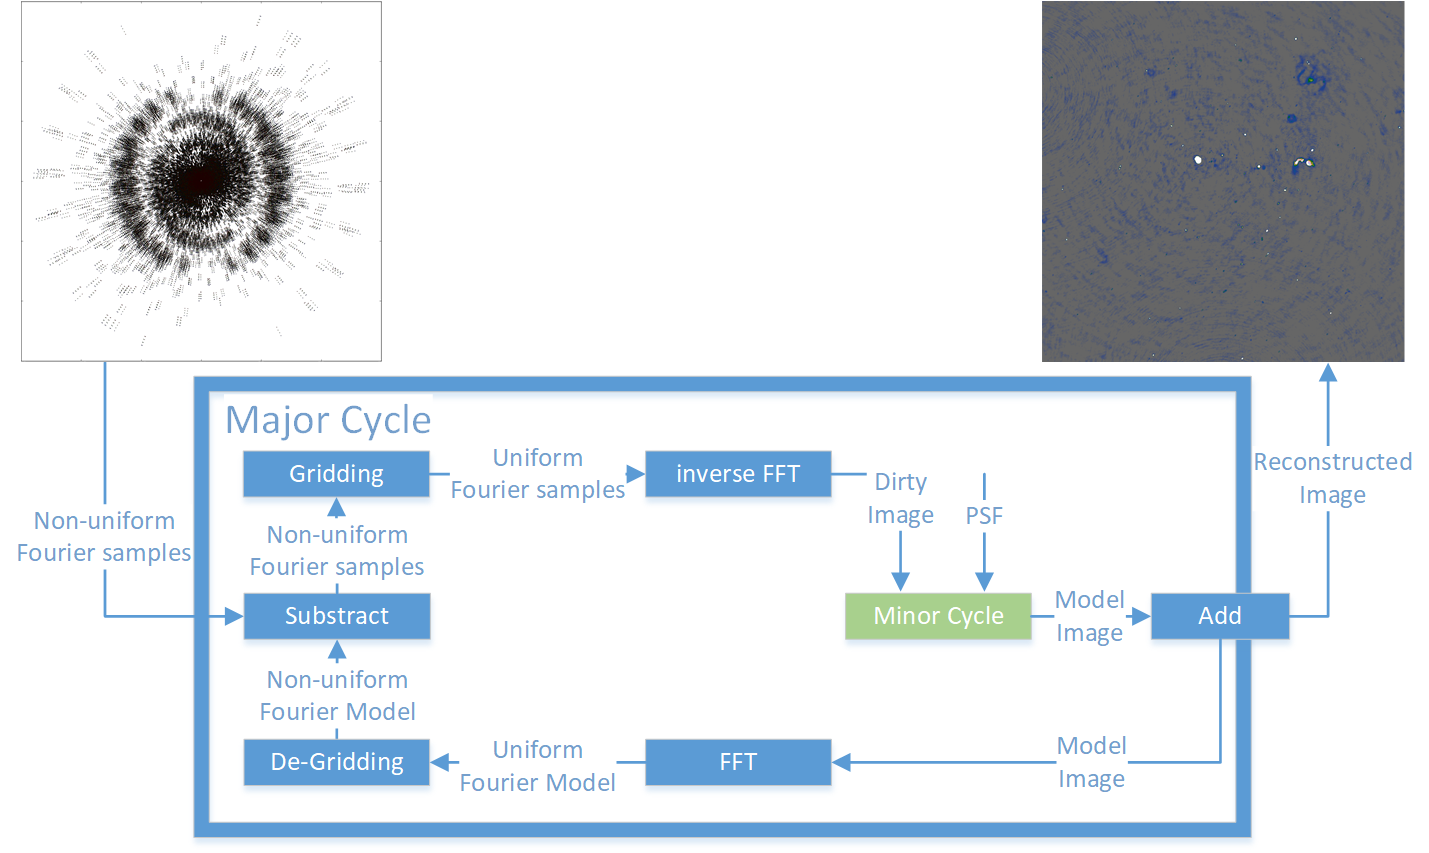
\includegraphics[width=0.80\linewidth]{./chapters/02.hypo/Major-Minor3.png}
	\caption{The Major Cycle Architecture}
	\label{intro:major}
\end{figure}

The Gridder + FFT is responsible for a fast approximation of $F$, while the deconvolution algorithm
Gridder is responsible for handling all Radio Interferometry weirdness. It has to handle the $w$-term of the Visibilities \eqref{intro:inverseproblem}. In practice, even more corrections fall onto the job of the Gridder. Since we have magnitudes more Visibilities than pixels, the Gridder's job is to "compress" the problem.

Note on the Cyclic Nature. It is counter intuitive and explained later in 

\subsubsection{The Gridder}


\subsubsection{Minor Cycle: CLEAN Deconvolutions}
Contains two classes of objects: Point sources, which are essentially stars, and extended emissions, which span over several pixels.


\subsubsection{Why are there Major Cycles in the first place?}
\begin{figure}[h]
	\centering
	\begin{subfigure}[b]{0.3\linewidth}
		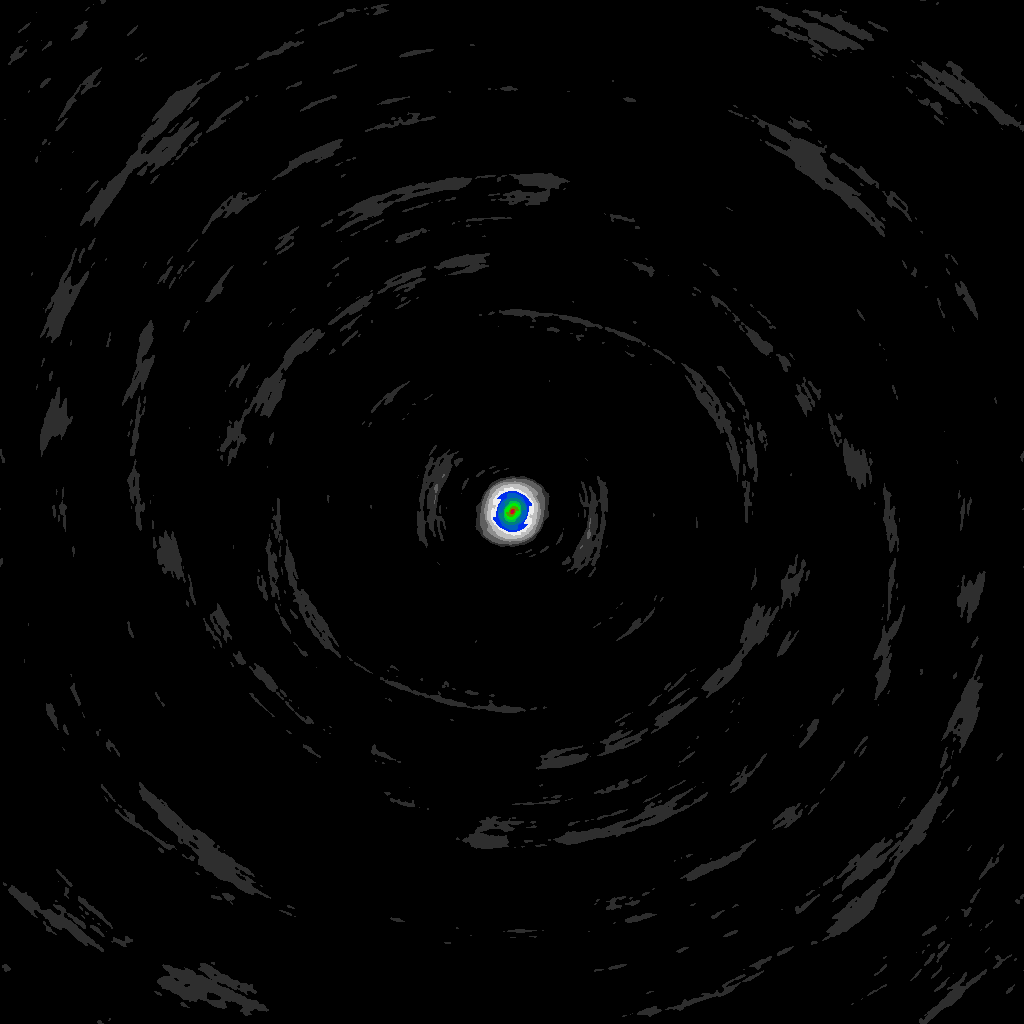
\includegraphics[width=\linewidth]{./chapters/01.intro/mk2/psf.png}
		\caption{Point Spread Function.}
		\label{results:points:tclean}
	\end{subfigure}
	\begin{subfigure}[b]{0.3\linewidth}
		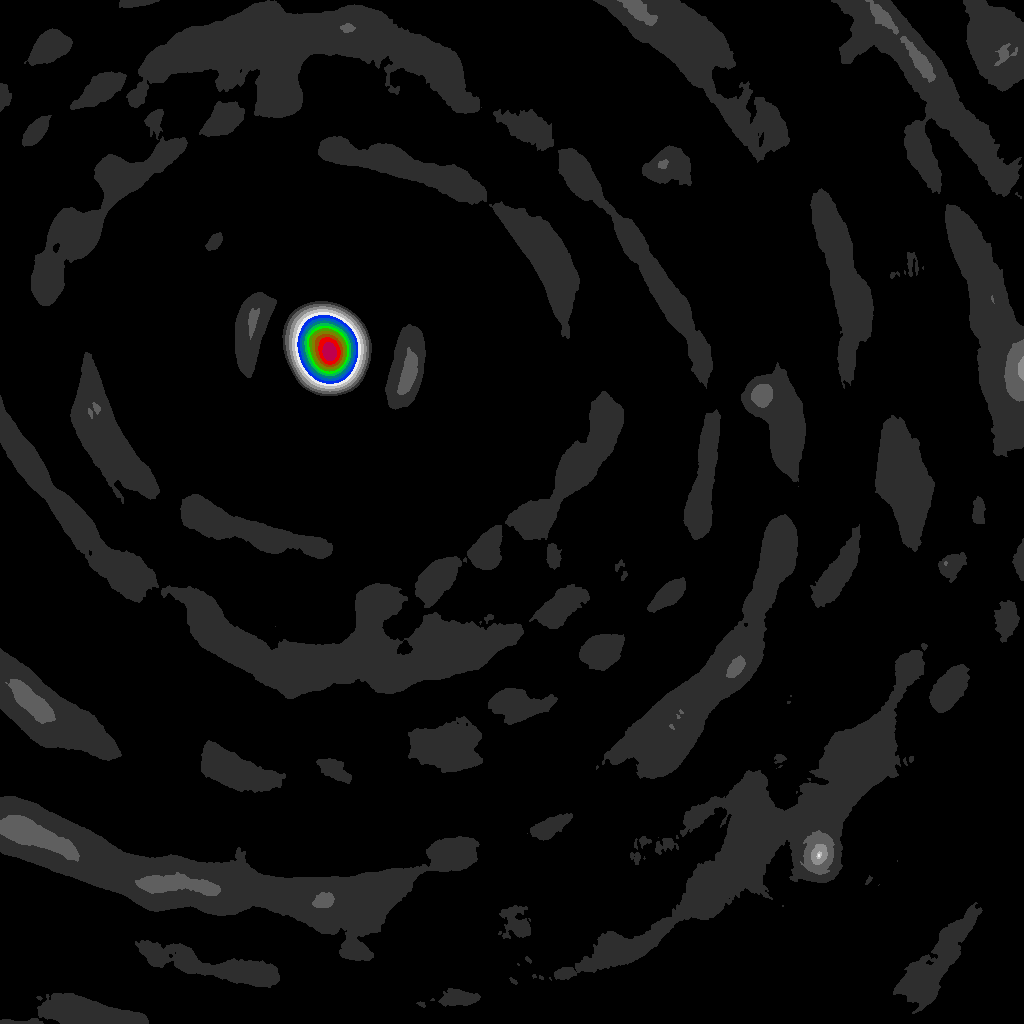
\includegraphics[width=\linewidth]{./chapters/01.intro/mk2/dirty.png}
		\caption{Dirty image}
		\label{results:points:tclean}
	\end{subfigure}
	\begin{subfigure}[b]{0.3\linewidth}
		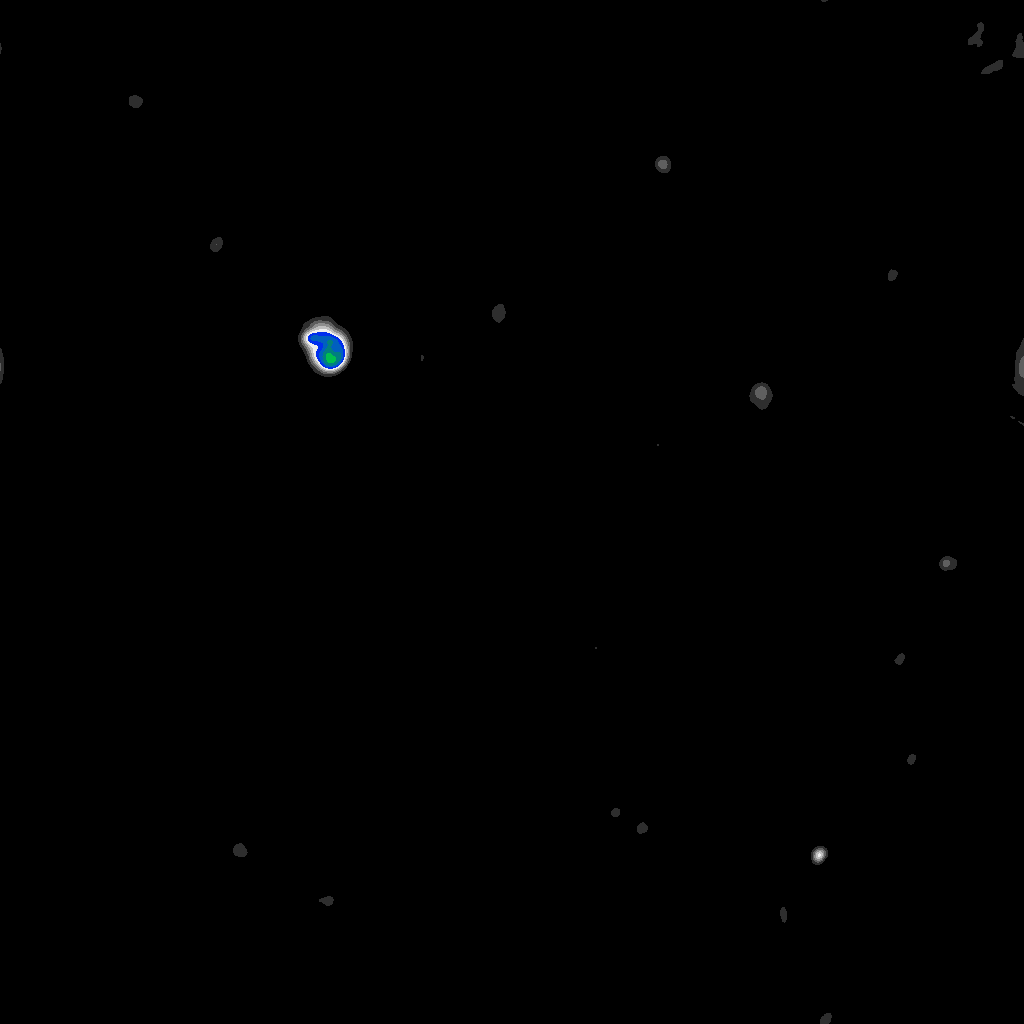
\includegraphics[width=\linewidth]{./chapters/01.intro/mk2/clean.png}
		\caption{Deconvolved image.}
		\label{results:points:tclean}
	\end{subfigure}
	
	
	\caption{Image reconstruction of two simulated point sources.}
	\label{results:points}
\end{figure}
Find the fainter sources in later iterations
Because we can only estimate the psf.



\subsection{Distributing the Major and Minor Cycles}
Difficulty in separation
Each Pixel depends on all Visibilities, and a single Visibility depends on all pixels.
Doing work several times

\subsubsection{Compressed Sensing and the evolution of Priors}
Positivity constraint.
Contains two classes of objects: Point sources, which are essentially stars, and extended emissions, which span over several pixels.


\subsection{The Major Cycle Architecture}
Major cycle how to reconstruct the image with deconvolution
In an efficient manner

$V()$ problems of non-uniform sampling, and the 3 dimensions. keep us from using the Fast Fourier Transform.
We first interpolate on a regularly spaced grid, in the "Gridder".
Use the FFT. For large numbers of Visibilities, this is faster. than inverting equation directly \eqref{intro:inverseproblem}.
And now we do a deconvolution in image space

So we have three basic components, Gridder, FFT and Deconvolution algorithms.
The Major Cycle Architecture makes this a cycle.
Shown in figure \ref{intro:major}.



Why the cycle is necessary



\subsubsection{Minor Cycle}


